% ------------------------------------------------------------------------------
% TYPO3 Version 9.3 - What's New - Chapter "Miscellaneous" (English Version)
%
% @author	Michael Schams <schams.net>
% @license	Creative Commons BY-NC-SA 3.0
% @link		http://typo3.org/download/release-notes/whats-new/
% @language	English
% ------------------------------------------------------------------------------
% LTXE-CHAPTER-UID:		68197358-0dc32ac8-dea3141e-8267c2d8
% LTXE-CHAPTER-NAME:	Miscellaneous
% ------------------------------------------------------------------------------

\section{Miscellaneous}
\begin{frame}[fragile]
	\frametitle{Miscellaneous}

	\begin{center}\huge{Chapter 5:}\end{center}
	\begin{center}\huge{\color{typo3darkgrey}\textbf{Miscellaneous}}\end{center}

\end{frame}

% ------------------------------------------------------------------------------
% LTXE-SLIDE-START
% LTXE-SLIDE-UID:		e53cbff2-1bede6e2-ad7f5aba-e91e7575
% LTXE-SLIDE-TITLE:		Argon2 Password Hashing Algorithm
% LTXE-SLIDE-REFERENCE:	#79889 - Saltedpasswords supports PHP password API
% ------------------------------------------------------------------------------

\begin{frame}[fragile]
	\frametitle{Miscellaneous}
	\framesubtitle{Argon2 Password Hashing Algorithm}

	\begin{itemize}
		\item System extension \texttt{EXT:saltedpasswords} now supports the
			\href{https://secure.php.net/manual/en/ref.password.php}{PHP Password Hashing API},
			which introduces the Argon2 hashing algorithm
		\item Integrators can choose between several password hashing methods
			for FE and BE user passwords
	\end{itemize}

	\begin{figure}
		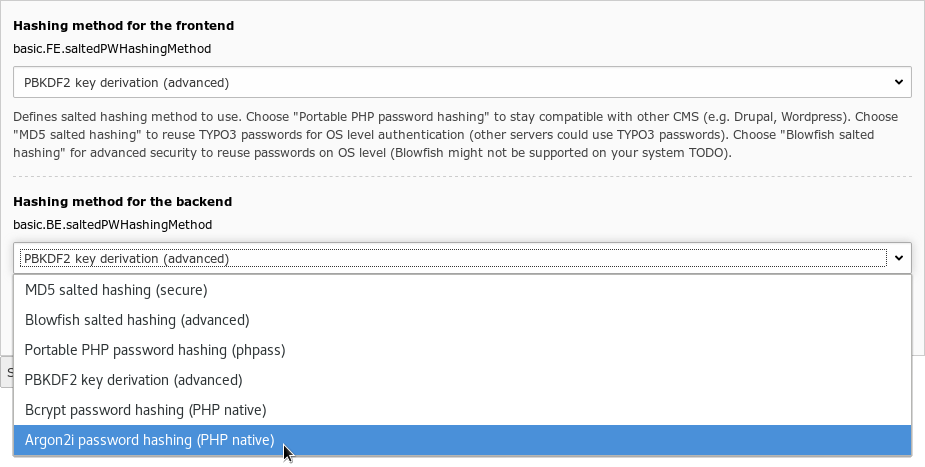
\includegraphics[width=0.65\linewidth]{Miscellaneous/SaltedPasswordsArgon2.png}
	\end{figure}

%	\begin{itemize}
%		\item Password hashes of existing users are automatically updated as required,
%			as soon as users log in
%	\end{itemize}

\end{frame}

% ------------------------------------------------------------------------------
% LTXE-SLIDE-START
% LTXE-SLIDE-UID:		e53cbff2-1bede6e2-ad7f5aba-e91e7575
% LTXE-SLIDE-TITLE:		Password Fields in the Install Tool
% LTXE-SLIDE-REFERENCE:	#81794 - Password fields in the Install tool
% ------------------------------------------------------------------------------

\begin{frame}[fragile]
	\frametitle{Miscellaneous}
	\framesubtitle{Install Tool Password Fields}

	\begin{itemize}
		\item Install Tool now supports password fields to prevent sensitive
			information to be shown
	\end{itemize}

	\tabto{0.3cm}For example field \texttt{Mail/transport\_smtp\_password}:

	\begin{figure}
		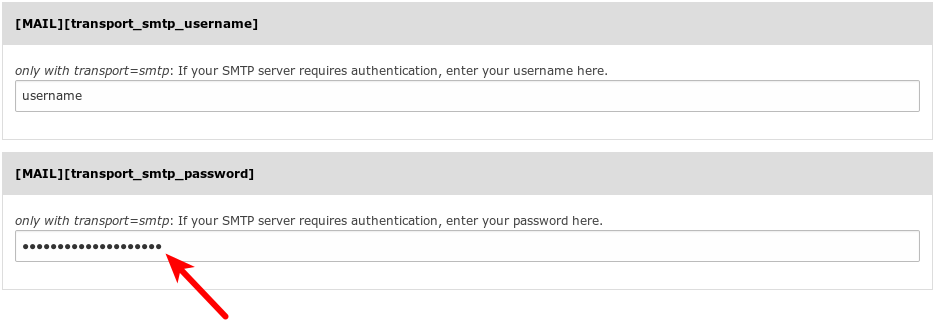
\includegraphics[width=0.95\linewidth]{Miscellaneous/InstallToolPasswordFields.png}
	\end{figure}

\end{frame}

% ------------------------------------------------------------------------------
